\documentclass[table]{beamer}

% Alternative to \usetheme{claw}
\usepackage{template/beamercolorthemeclaw}
\usepackage{template/beamerfontthemeclaw}
\usepackage{template/beamerinnerthemeclaw}
\usepackage{template/beamerouterthemeclaw}

\usepackage{standalone}
\usepackage{booktabs}
%\usepackage{hhline}
\usepackage{lmodern}


\definecolor{tab20darkblue}{HTML}{4e79a7}
\definecolor{tab20darkgreen}{HTML}{59a14f}
\definecolor{tab20darkred}{HTML}{e15759}
\definecolor{tab20darkorange}{HTML}{f28e2b}
\definecolor{tab20darkturquoise}{HTML}{499894}
\definecolor{tab20darkgray}{HTML}{79706e}
\definecolor{tab20darkbrown}{HTML}{9d7660}
\definecolor{tab20darkpurple}{HTML}{b07aa1}
\definecolor{tab20darkpink}{HTML}{e377c2}
\definecolor{tab20lightgreen}{HTML}{8cd17d}
\definecolor{tab20lightblue}{HTML}{a0cbd8}
\definecolor{tab20lightorange}{HTML}{ffbb78}
\definecolor{tab20lightred}{HTML}{ff9896}
\definecolor{tab20lightpurple}{HTML}{c5b0d5}
\definecolor{tab20lightbrown}{HTML}{c49c94}
\definecolor{tab20lightpink}{HTML}{f7b6d2}
\definecolor{tab20lightgray}{HTML}{c7c7c7}
\definecolor{tab20lightturquoise}{HTML}{9edae5}
\definecolor{tab20lightyellow}{HTML}{dbdb8d}
\definecolor{tab20darkyellow}{HTML}{bcbd22}

\definecolor{brass}{HTML}{E1C16E}



% Configuration

% Path for images
\graphicspath{{./images/}}

% OPTIONAL: Insert additional slide at begin of each section
%\AtBeginSection{\frame{\sectionpage}}

% OPTIONAL: Background image with logos
\usebackgroundtemplate{
\includegraphics[width=\paperwidth]{background-upb-dice}}
% German UPB logo
%\usebackgroundtemplate{
\includegraphics[width=\paperwidth]{background-upb-dice-german}}
% Reduce max. frame title width (no logo overlap)
\renewcommand{\frametitlewidth}{.8\textwidth}

% OPTIONAL: Replace blue with specific blue
\colorlet{textblue}{textbluespecific}
\colorlet{elementblue}{elementbluespecific}
\colorlet{lightblue}{lightbluespecific}
\colorlet{backgroundblue}{backgroundbluespecific}

% OPTIONAL: Less space inside blocks
% https://tex.stackexchange.com/a/94189
%\makeatletter
%\addtobeamertemplate{block begin}{
%\def\@listi{\leftmargin\leftmargini
%\topsep    0pt
%\parsep    0pt
%\itemsep   3pt plus 2pt minus 3pt}
%\partopsep 0pt }
%\makeatother
%\makeatletter
%\addtobeamertemplate{block example begin}{
%\def\@listi{\leftmargin\leftmargini
%\topsep    0pt
%\parsep    0pt
%\itemsep   3pt plus 2pt minus 3pt}
%\partopsep 0pt }
%\makeatother
%\makeatletter
%\addtobeamertemplate{block alerted begin}{
%\def\@listi{\leftmargin\leftmargini
%\topsep    0pt
%\parsep    0pt
%\itemsep   3pt plus 2pt minus 3pt}
%\partopsep 0pt }
%\makeatother


% Packages

% inputenc - Accept different input encodings
% https://ctan.org/pkg/inputenc
\usepackage[utf8x]{inputenc}

% babel - Multilingual support for Plain TEX or LATEX
% https://ctan.org/pkg/babel
\usepackage[english]{babel}
%\usepackage[german]{babel}

% hyperref – Extensive support for hypertext in LATEX
% https://ctan.org/pkg/hyperref
\usepackage{hyperref}
\hypersetup{
	colorlinks=true,
	linkcolor=footertext,
	urlcolor=urls
}

% appendixnumberbeamer – Manage frame numbering in appendixes in beamer
% https://ctan.org/pkg/appendixnumberbeamer
\usepackage{appendixnumberbeamer} 


\usepackage[absolute,overlay]{textpos}
\usepackage{multicol}

\usepackage{mathtools}
\usepackage{amsmath,amssymb}
% Fonts
% https://tug.org/FontCatalogue/
% https://ctan.org/pkg/free-math-font-survey

% fontenc – Standard package for selecting font encodings
% https://ctan.org/pkg/fontenc
\usepackage[T1]{fontenc}

% Serif font
\usepackage{bera}

% Mono font
\usepackage{nimbusmononarrow}

% Sans-Serif font (fallback)
% tgheros
\usepackage{tgheros}

% Font Roboto Condensed
% https://tug.org/FontCatalogue/robotocondensed/
% https://ctan.org/pkg/roboto
\usepackage[sfdefault,condensed]{roboto}

% Alternative: Arial Narrow
% Fontspec requires XeTeX or LuaTeX, not PDFLaTeX
%\usepackage{fontspec}
%\setsansfont[Ligatures=TeX]{Arial Narrow}



% Optional packages
% Can be removed if not used

% pgf – Create PostScript and PDF graphics in TEX
% https://www.ctan.org/pkg/pgf
\usepackage{tikz}
\usetikzlibrary{shapes,positioning}
\usetikzlibrary{arrows.meta,arrows}
\tikzset{resource/.style={draw,rectangle,fill=lightblue,rounded corners,inner sep=5pt} }
\tikzset{literal/.style={draw,rectangle,fill=lightyellow,inner sep=5pt}}
\tikzset{>=triangle 45}
\tikzset{every picture/.style=thick}
\tikzstyle{every node}=[font=\small]

% listings – Typeset source code listings using LATEX
% https://ctan.org/pkg/listings
\usepackage{listings}
\lstset{
	basicstyle=\small\ttfamily,
	%
	keywordstyle=\color{textblue},
	commentstyle=\color{textgray},
	emphstyle=\color{textpurple},
	%
	numbers=left,
	numbersep=7pt,
	numberstyle=\scriptsize\color{textgray}\ttfamily,
	%
	tabsize=2,
	breaklines=true
}



% Beamer settings

% Disable navigation symbols
\setbeamertemplate{navigation symbols}{}

% Move title page contents down
\addtobeamertemplate{title page}{\vspace{2\baselineskip}}{}

% OPTIONAL: Alternative footer
%\useoutertheme{infolines}
%\setbeamertemplate{headline}{}
%\setbeamerfont{title in head/foot}{series=\mdseries}

% OPTIONAL: Alternative header/footer colors
%\setbeamercolor{palette primary}{bg=lightgray}
%\setbeamercolor{palette secondary}{bg=lightgray}
%\setbeamercolor{palette tertiary}{bg=lightgray}
%\setbeamercolor{frametitle}{bg=lightgray}



% Commands

% Text color
\newcommand{\bluedark}[1]{\textcolor{textbluedark}{#1}}
\newcommand{\blue}[1]{\textcolor{textblue}{#1}}
\newcommand{\gray}[1]{\textcolor{textgray}{#1}}
%
\newcommand{\magenta}[1]{\textcolor{textmagenta}{#1}}
\newcommand{\orange}[1]{\textcolor{textorange}{#1}}
\newcommand{\purple}[1]{\textcolor{textpurple}{#1}}
%
\newcommand{\red}[1]{\textcolor{textred}{#1}}
\newcommand{\turquoise}[1]{\textcolor{textturquoise}{#1}}
\newcommand{\green}[1]{\textcolor{textgreen}{#1}}

% Predefined text concepts
\renewcommand{\alert}[1]{\textbf{\red{#1}}}
\renewcommand{\emph}[1]{\blue{#1}}
\newcommand{\good}[1]{\turquoise{#1}}
\newcommand{\bad}[1]{\purple{#1}}

\newcommand{\heading}[1]{\textbf{#1}\\\vspace*{.05cm}}
\newcommand{\tech}[1]{\gray{\texttt{#1}}}
\newcommand{\term}[1]{\gray{\textit{#1}}}

% OPTIONAL: Example blocks in green instead of turquoise
%\setbeamercolor{block title example}{bg=lightgreen,fg=templatetext}
%\setbeamercolor{block body example}{bg=backgroundgreen}
% OPTIONAL: Positive highlights in green instead of turquoise
%\renewcommand{\good}[1]{\green{#1}}

% OPTIONAL: Alert blocks in red instead of purple
%\setbeamercolor{block title alerted}{bg=lightred,fg=templatetext}
%\setbeamercolor{block body alerted}{bg=backgroundred}
% OPTIONAL: Negative highlights in red instead of purple
%\renewcommand{\bad}[1]{\red{#1}}

% OPTIONAL: Alert blocks in magenta instead of purple
%\setbeamercolor{block title alerted}{bg=lightmagenta,fg=templatetext}
%\setbeamercolor{block body alerted}{bg=backgroundmagenta}
% OPTIONAL: Negative highlights in magenta instead of purple
%\renewcommand{\bad}[1]{\magenta{#1}}


% Figures.
\usepackage{tikz-qtree}
\usepackage{pgfplots}
\pgfplotsset{compat=1.16}
\usetikzlibrary{shapes, positioning, arrows}



% 1st used for slides footer, 2nd for title slide & PDF metadata
\title[CausalQA]{Answering Causal Questions With Reinforcement Learning}
% Used for title slide & PDF metadata
\subtitle{}

%\date{April 27, 2022}
% Date with conference name
\date[\today]

% One author
% 1st used for slides footer, 2nd for title slide & PDF metadata
\author[Lukas Blübaum]{Lukas Blübaum \\ \vspace{0.5cm}Supervisor: Dr. Stefan Heindorf}

% 1st used for slides footer, 2nd for title slide
%\institute[DICE]{DICE Group\\Paderborn University}
% Institute with logo
\institute[DICE]{
\includegraphics[height=0.6cm]{DICE}\\Data Science Group\\Paderborn University}

% Two authors from different institutes
% Source: https://www.overleaf.com/learn/latex/Beamer#The_title_page
%\author[\underline{Wilke}, Ngonga]{\underline{Adrian~Wilke}\inst{1} \and Axel~Ngonga\inst{2}}
%\institute[]
%{
%	\inst{1}%
%	DICE Group\\
%	Department of Computer Science\\
%	Paderborn University, Germany
%	\and
%	\inst{2}%
%	DICE Group\\
%	Department of Computer Science\\
%	Paderborn University, Germany
%}

% One logo on title page
%\titlegraphic{
\includegraphics[height=1cm]{DICE}}

% Two logos on title page
%\titlegraphic{
%	
\includegraphics[height=1cm]{UPB}%
%	\hspace*{2cm}~%
%	
\includegraphics[height=1cm]{DICE}%
%}

% Siavoosh Payandeh Azad Jan. 2019
\RequirePackage{etoolbox}
\RequirePackage{pgf} % for calculating the values for gradient
\RequirePackage{xcolor} % enables the use of cellcolor make sure you have [table] option in the document class 
% Color set related!
%\definecolor{high}{HTML}{ef3b2c}  % the color for the highest number in your data set
%\definecolor{high}{HTML}{b9f3be}
\definecolor{high}{HTML}{8cd17d}
%\definecolor{low}{HTML}{ef3b2c}
%\definecolor{low}{HTML}{ff9896}
%\definecolor{low}{HTML}{f79e4c}
%\definecolor{low}{HTML}{fbd769}
\definecolor{low}{HTML}{faf2a7}
%\definecolor{low}{HTML}{fff7bc}  % the color for the lowest number in your data set
\newcommand*{\opacity}{90}% here you can change the opacity of the background color!
%======================================
% Data set related!
\newcommand*{\minval}{0.38}% define the minimum value on your data set
\newcommand*{\maxval}{1.0}% define the maximum value in your data set!
%======================================
% gradient function!
\newcommand{\g}[1]{%
    % The values are calculated linearly between \minval and \maxval
    \ifdimcomp{#1pt}{>}{\maxval pt}{#1}{%
    \ifdimcomp{#1pt}{<}{\minval pt}{#1}{%
         \pgfmathparse{int(round(100*(#1/(\maxval-\minval))-(\minval*(100/(\maxval-\minval)))))}%
        \xdef\tempa{\pgfmathresult}%
        \cellcolor{high!\tempa!low!\opacity}%
    }}%
 }%
%======================================
% gradient function single cell! 
\newcommand{\gradientcell}[6]{
    % The values are calculated linearly between \minval and \maxval
    \ifdimcomp{#1pt}{>}{#3 pt}{#1}{
    \ifdimcomp{#1pt}{<}{#2 pt}{#1}{
         \pgfmathparse{int(round(100*(#1/(#3-#2))-(\minval*(100/(#3-#2)))))}
        \xdef\tempa{\pgfmathresult}
        \cellcolor{#5!\tempa!#4!#6} #1
    }}
 }

\pdfsuppresswarningpagegroup=1

\begin{document}

% Title page without background
%{\usebackgroundtemplate{}
%\frame[plain]{\titlepage}}

% Title page with background
{\usebackgroundtemplate{
\includegraphics[width=\paperwidth]{background-title-upb}
% German UPB logo
%\usebackgroundtemplate{
\includegraphics[width=\paperwidth]{background-title-upb-german}
}
\frame[plain]{\titlepage}}

% Begin counting at second frame
\addtocounter{framenumber}{-1}


\begin{frame}{Causal Question Answering}
  \begin{columns}[T]
    \column{0.62\textwidth}
  \begin{itemize}
    \item<1-> Causal Questions
    \begin{itemize}
      \item Determine relationships between causes and effects
      \item E.g. understand what effects a cause could have in the future
    \end{itemize}
    \item<2-> Use Cases
    \begin{itemize}
      \item Search engines
      \item Virtual assistants like Alexa
      \item Automated decision-making
    \end{itemize}
    \item<3-> Limitations of prior approaches
    \begin{itemize}
      \item Often \emph{not explainable}
      \item \emph{Lack of large-scale datasets} of causal relations of high quality
    \end{itemize}
  \end{itemize}
  \column{0.38\textwidth}
  
  \scriptsize
  \emph{\textbf{Binary Causal Questions}}\\
  \emph{Does pneumonia cause anemia?}\\
  \vspace{0.2cm}
  \textbf{Open-Ended Questions}\\
  What can cause anemia?\\
  \vspace{0.2cm}
  \textbf{Comprehension Questions}\\
  How does pneumonia cause anemia?
  %\textbf{Open-Ended Questions}\\
  %What can cause anemia?\\\\
  %\textbf{More complex questions}\\
  %How does pneumonia cause anemia?
  %\begin{textblock*}{5cm}(9cm,1.8cm) 
  %\resizebox{0.7\textwidth}{!}{
  %\begin{tikzpicture}
    %\node[object, xshift=2cm,yshift=2cm, anchor=north east] (P1) {organ failure};
    %\node[object,xshift=2cm,yshift=2cm, anchor=north east, fill=tab20darkred!60,label={0: \huge $\mathbf{\downarrow}$}] (P2) {climate change};
    %\node[object, right= 0.5cm of P2] (P3) {ards};
    
   % \node (T1) {\textbf{Binary Causal Questions}};
   % \node[below = 0.3cm of T1] (T2) {Does pneumonia cause anemia?};

   \tikzset{person/.style={draw,rectangle,fill=tab20darkgreen!60,rounded corners,inner sep=5pt} }
  \tikzset{object/.style={draw,rectangle,fill=tab20darkblue!60,rounded corners, inner sep=5pt, minimum height=0.7cm}}
  \tikzset{type/.style={draw,rectangle,fill=lightgray,inner sep=5pt}}
  \tikzset{>=triangle 45}
  \tikzset{every picture/.style=thick}
  \tikzstyle{every node}=[font=\small]
    \tikzstyle{arrow} = [->, thick,>=stealth']
  
  
  \vspace{-0.5cm}
  \begin{textblock*}{5cm}(8cm,5.0cm) 
    \resizebox{0.7\textwidth}{!}{%
  \hspace{0.0cm}
  \begin{tikzpicture}
    \node[object, fill=white] (P1) {sepsis};
    \node[object, right= 0.5cm of P1] (P2) {anemia};
    \node[object, right= 0.5cm of P2, fill=white] (P3) {ards};
    
    \node[person, above=of P2] (T1) {pneumonia};

    \draw[arrow, line width=1.2pt] (T1) -- (P1);
    \draw[arrow, line width=1.2pt] (T1) -- (P2);
    \draw[arrow, line width=1.2pt] (T1) -- (P3);

  \end{tikzpicture}}
  \end{textblock*}
  %\end{tikzpicture}}
  %\end{textblock*}
  \end{columns}
\end{frame}

\begin{frame}{Causal Question Answering}
  \begin{itemize}
    \item<1-> Solution
    \begin{itemize}
      \item Perform \emph{walks on a knowledge graph}
      \item Formulated as a sequential decision problem\\via reinforcement learning
    \end{itemize}
    \item<2-> Advantages
    \begin{itemize}
      \item Answers are \emph{explainable}\\$\Rightarrow$ Can follow the reasoning chain
      \item Can answer \emph{binary and open-ended questions}
      %\item Performs better than walks learned\\via supervised learning
    \end{itemize}
    \item<3-> Contributions
    \begin{itemize}
      \item Approach to answer \emph{binary causal questions}\\via reinforcement learning
      \item Introduce an Actor-Critic (A2C) based agent with\\generalized advantage estimation (GAE)
      \item Supervised learning and reward shaping to deal with\\large action spaces and sparse rewards
    \end{itemize}
  \end{itemize}
   \tikzset{person/.style={draw,rectangle,fill=tab20darkgreen!60,rounded corners,inner sep=5pt, minimum height=0.7cm} }
  \tikzset{object/.style={draw,rectangle,fill=tab20darkgreen!60,rounded corners, inner sep=5pt, minimum height=0.7cm}}
  \tikzset{type/.style={draw,rectangle,fill=lightgray,inner sep=5pt}}
  \tikzset{>=triangle 45}
  \tikzset{every picture/.style=thick}
  \tikzstyle{every node}=[font=\small]
    \tikzstyle{arrow} = [->, thick,>=stealth']

  \begin{textblock*}{5cm}(9cm,1.8cm) 
  \resizebox{0.7\textwidth}{!}{
  \begin{tikzpicture}[remember picture]
    
    \node[object, xshift=2cm,yshift=2.2cm, anchor=north east] (P1) {fatigue};
    \node[object, right= 0.7cm of P1,fill=tab20darkblue!60] (P2) {sepsis};
    \node[object, right= 0.7cm of P2] (P3) {ards};
    
    \node[person, above=0.7cm of P2,fill=tab20darkblue!60] (T1) {pneumonia};
    \node[person, above=0.7cm of T1] (T2) {bacteria};
    \node[person, below=0.7cm of P3] (T3) {death};
    \node[person, below=0.7cm of T3] (P8) {grief};
    \node[person, below=0.7cm of P2,fill=tab20darkblue!60] (T4) {kidney failure};
    \node[person, below=0.7cm of T4,fill=tab20darkblue!60] (P7) {anemia};

    \node[above=0.7cm of T2] (T5) {\textbf{Does pneumonia cause anemia?}};

    \draw[arrow, line width=1.2pt] (T1) -- (P1);
    \draw[arrow, line width=1.2pt] (T1) -- (P2);
    \draw[arrow, line width=1.2pt] (T1) -- (P3);
    \draw[arrow, line width=1.2pt] (T2) -- (T1);
    \draw[arrow, line width=1.2pt] (P3) -- (T3);
    \draw[arrow, line width=1.2pt] (P2) -- (T4);
    \draw[arrow, line width=1.2pt] (T4) -- (P7);
    \draw[arrow, line width=1.2pt] (T3) -- (P8);

  \end{tikzpicture}}
  \end{textblock*}
\end{frame}


\begin{frame}{CauseNet}{Large-Scale Causal Knowledge Graph}
  \begin{itemize}
	  \item $\mathcal{K}=(\mathcal{E}, \mathcal{R})$: entities $\mathcal{E}$, relations $\mathcal{R}$
	  \item $\mathcal{R} = \{mayCause\}$:\\$\Rightarrow$ Claimed causal relations
	  %\item Extracted via linguistic pattern from\\web sources like Wikipedia and ClueWeb12
    \item Meta-information like the \emph{original sentence} \\and the \emph{URL} for each relation
	  \item Two configurations: \emph{CauseNet-Precision}\\and CauseNet-Full~{\scriptsize\cite{Heindorf2020Causenet}}
\end{itemize}

   \tikzset{person/.style={draw,rectangle,fill=tab20darkgreen!60,rounded corners,inner sep=5pt, minimum height=0.7cm} }
  \tikzset{object/.style={draw,rectangle,fill=tab20darkgreen!60,rounded corners, inner sep=5pt, minimum height=0.7cm}}
  \tikzset{type/.style={draw,rectangle,fill=lightgray,inner sep=5pt}}
  \tikzset{>=triangle 45}
  \tikzset{every picture/.style=thick}
  \tikzstyle{every node}=[font=\small]
    \tikzstyle{arrow} = [->, thick,>=stealth']
  
  

  \begin{textblock*}{5cm}(8.4cm,1.5cm) 
  \resizebox{0.8\textwidth}{!}{
  \begin{tikzpicture}[remember picture]
    \node[object, xshift=2cm,yshift=2cm, anchor=north east] (P1) {sepsis};
    \node[object, right= 0.5cm of P1] (P2) {anemia};
    \node[object, right= 0.5cm of P2] (P3) {ards};
    
    \node[person, above=0.7cm of P2] (T1) {pneumonia};
    \node[person, above=0.7cm of T1] (T2) {bacteria};
    \node[person, below=0.7cm of P3] (T3) {death};
    \node[person, below=0.7cm of P2] (T4) {fatigue};

    \draw[arrow, line width=1.2pt] (T1) -- (P1);
    \draw[arrow, line width=1.2pt] (T1) -- (P2);
    \draw[arrow, line width=1.2pt] (T1) -- (P3);
    \draw[arrow, line width=1.2pt] (T2) -- (T1);
    \draw[arrow, line width=1.2pt] (P3) -- (T3);
    \draw[arrow, line width=1.2pt] (P2) -- (T4);

  \end{tikzpicture}}
\end{textblock*}

	\begin{exampleblock}<2->{Causal Questions}
	\begin{itemize}
	  \item Does \underline{pneumonia} cause \underline{fatigue}?
	  \item Is \underline{sepsis} caused by \underline{pneumonia}?
	\end{itemize}
\end{exampleblock}

\end{frame}

\begin{frame}{Task and Problem Definition}
	\begin{block}{Causal Question Answering on Knowledge Graph $\mathcal{K}$}
    \begin{itemize}
	\item Input:
	\begin{itemize}
	  \item $\mathcal{K}=(\mathcal{E}, \mathcal{R})$ with $\mathcal{R} = \{cause\}$
    \item Question $q$ with exactly \emph{one cause} $e_c$ and \emph{one effect} $e_e$\\
    \textcolor{gray}{Does pneumonia ($= e_c$) cause anemia ($ = e_e$)?}
	\end{itemize}
	\item<2-> Output:
	\begin{itemize}
	    \item Path: $(e_c, e_1, \dots, e_e)$ with $e_c, e_i, e_e \in \mathcal{E}$
      \item If such a path can be found answer ``yes'' and ``no'' otherwise
    \end{itemize}
	\item<3-> Challenges:
	\begin{itemize}
	    \item Only \emph{one relation type} contrary to prior approaches\\$\Rightarrow$ Large action space
	    \item CauseNet-Precision has 80,223 entities
    \end{itemize}
  \end{itemize}
\end{block}
\end{frame}

\begin{frame}{Reinforcement Learning}
\begin{itemize}
  \item Policy gradient methods with policy network $\pi_{\theta} (a_t | s_t)$:
  \begin{equation*}
    \nabla_{\theta} J (\theta) = \mathbb{E}_{\pi_\theta} \left[ \sum_{t=0}^T \nabla_\theta \, \log(\pi_\theta (a_t | s_t)) \Psi_t \right] 
    \label{eq:polupdate}
  \end{equation*}
  \item<2-> Possible forms for $\Psi_t$~{\scriptsize\cite{Schulman2016GAE}}:
    \begin{equation*}
    R_t = \sum_{i=0}^{T-t} \gamma^{i} \, r_{t+i} \ \ \ \ \ \ \ \ \ \ \ \ \
      \mathcal{A}_t^\psi = R_t(\lambda) - V_\psi(s_t)
    \end{equation*}
  \item<3-> \emph{Monte-Carlo return} $R_t$ unbiased but high variance\\$\Rightarrow$ REINFORCE
  \item<3-> \emph{Advantage} $\mathcal{A}_t^{\psi}$ introduces value network $V_{\psi}(s_t)$ to \emph{reduce variance}\\$\Rightarrow$ Advantage Actor-Critic (A2C)~{\scriptsize\cite{Mnih2016A2C}}
  \item<3-> Using the $\lambda$-return $R_t(\lambda)$ in the advantage yields the generalized advantage estimation (GAE)~{\scriptsize\cite{Schulman2016GAE}}
\end{itemize}

\end{frame}

\begin{frame}{Environment}{Agent, States, Actions}
  \begin{columns}[T]
    \column{0.6\textwidth}
  \begin{itemize}
    \item Agent
    \begin{itemize}
      \item $\pi_\theta(a_t | s_t)$: policy network\\
       $\Rightarrow$ Distribution over actions
      \item $V_\psi(s_t)$: value network \\
      $\Rightarrow$ Reward from state $s_t$ onwards
    \end{itemize}
    \item<2-> States
    \begin{itemize}
      \item $s = (\mathbf{q}, e_t, \mathbf{e_t}, \mathbf{h_t}, e_e)$
      \item Question Embedding $\mathbf{q}$
      \item Current entity $e_t$, target entity $e_e$
      \item History $\mathbf{h_t}$ (LSTM hidden states)
    \end{itemize}
    \item<3-> Actions
    \begin{itemize}
      \item All neighboring entities of $e_t$:\\
      $A(s_t) = \{e | (e_t, r, e) \in \mathcal{K}\}$
    \end{itemize}
  \end{itemize}
  \column{0.4\textwidth}
  %\vspace{-1.0cm}
  \begin{figure}
    \centering
  \hspace*{-0.5cm}
  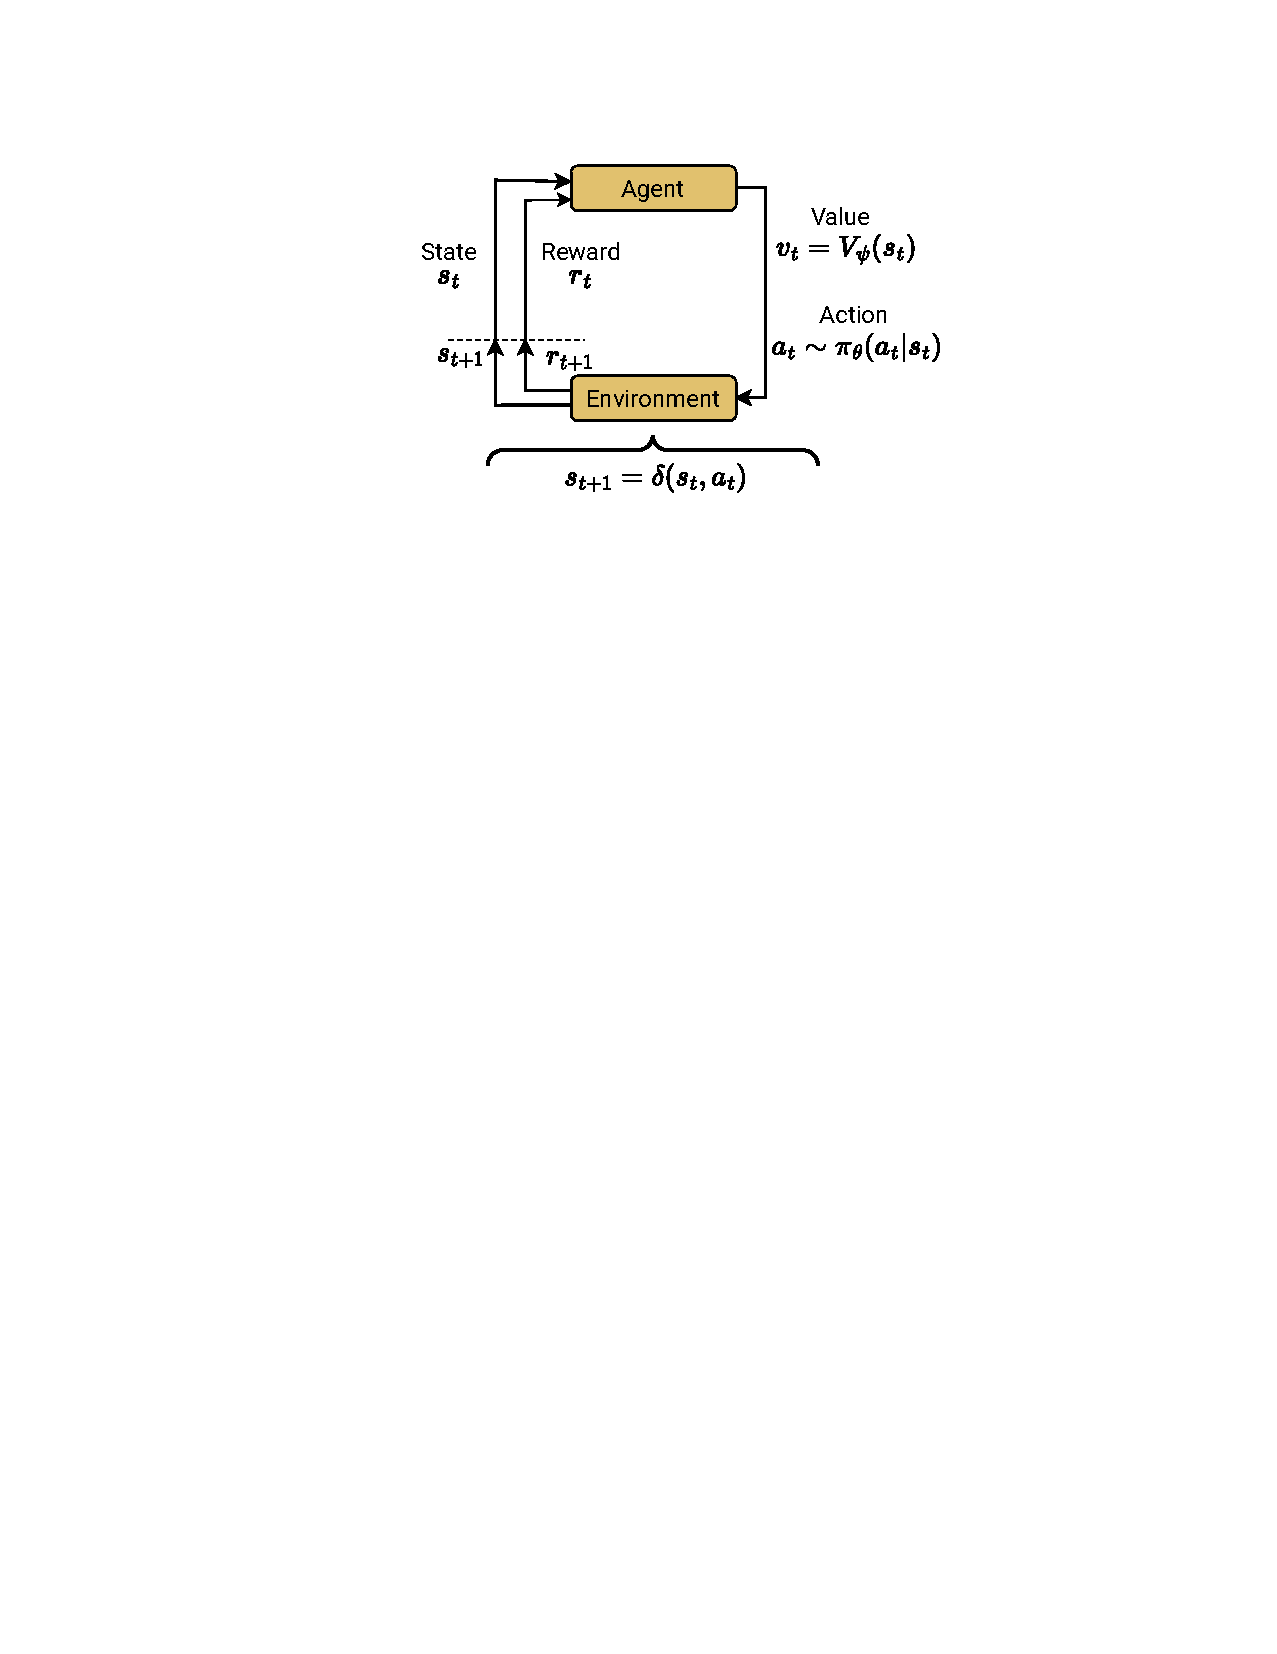
\includegraphics[clip, trim=7cm 19cm 5cm 2cm, width=1.3\textwidth]{rl.pdf}
  \end{figure}
   \tikzset{person/.style={draw,rectangle,fill=tab20darkgreen!60,rounded corners,inner sep=5pt} }
  \tikzset{object/.style={draw,rectangle,fill=tab20darkblue!60,rounded corners, inner sep=5pt, minimum height=0.7cm}}
  \tikzset{type/.style={draw,rectangle,fill=lightgray,inner sep=5pt}}
  \tikzset{>=triangle 45}
  \tikzset{every picture/.style=thick}
  \tikzstyle{every node}=[font=\small]
    \tikzstyle{arrow} = [->, thick,>=stealth']
  
  
  \vspace{-0.5cm}
    \resizebox{1.1\textwidth}{!}{%
  \hspace{0.0cm}
  \begin{tikzpicture}
    \node[object] (P1) {sepsis};
    \node[object, right= 0.5cm of P1, label={-90:$\mathbf{a_t = e_{t+1}}$}] (P2) {anemia};
    \node[object, right= 0.5cm of P2] (P3) {ards};
    \node[right= 0.1cm of P3] (P4) {\large $\biggl\} \, \, A(s_t)$};
    
    \node[person, above=of P2, label={90:$\mathbf{e_t}$}] (T1) {pneumonia};

    \draw[arrow, line width=1.2pt] (T1) -- (P1);
    \draw[arrow, line width=1.2pt] (T1) -- (P2);
    \draw[arrow, line width=1.2pt] (T1) -- (P3);

  \end{tikzpicture}}
  \end{columns}
\end{frame}

\begin{frame}{Environment}{Actions, Transitions, Rewards}
  \begin{columns}[T]
    \column{0.60\textwidth}
  \begin{itemize}
    \item Actions
    \begin{itemize}
      \item \textit{STAY} action: $A(s_t) = A(s_t) \cup \{STAY\}$
      \item Including \emph{inverse edges}
      %\item Embeddings: $\mathbf{a_t} = [\mathbf{s};\mathbf{a_t}]$ with\\original sentence $s$
    \end{itemize}
    \item<2-> Transitions
    \begin{itemize}
      \item $\delta(s_t, a_t) = s_{t+1}$ where $a_t = e_{t+1}$
      \item \emph{Deterministic} and entirely defined\\by the graph
    \end{itemize}
    \item<3-> Rewards
    \begin{itemize}
      \item $\mathcal{R}(s_{T-1}) = r_t$ with $r_t = 1$ if \emph{$e_{T-1} = e_e$} and $r_t = 0$ otherwise
      %$s_{T-1} = (\mathbf{q}, e_{T-1}, \mathbf{e_{T-1}}, \mathbf{h_{T-1}}, e_e)$ with 
      \item $0$ at all other time steps\\
      $\Rightarrow$ \emph{sparse reward}
    \end{itemize}
  \end{itemize}
  \column{0.4\textwidth}
  
  %\vspace{-0.2cm}
  \begin{figure}
    \centering
  \hspace*{-0.5cm}
  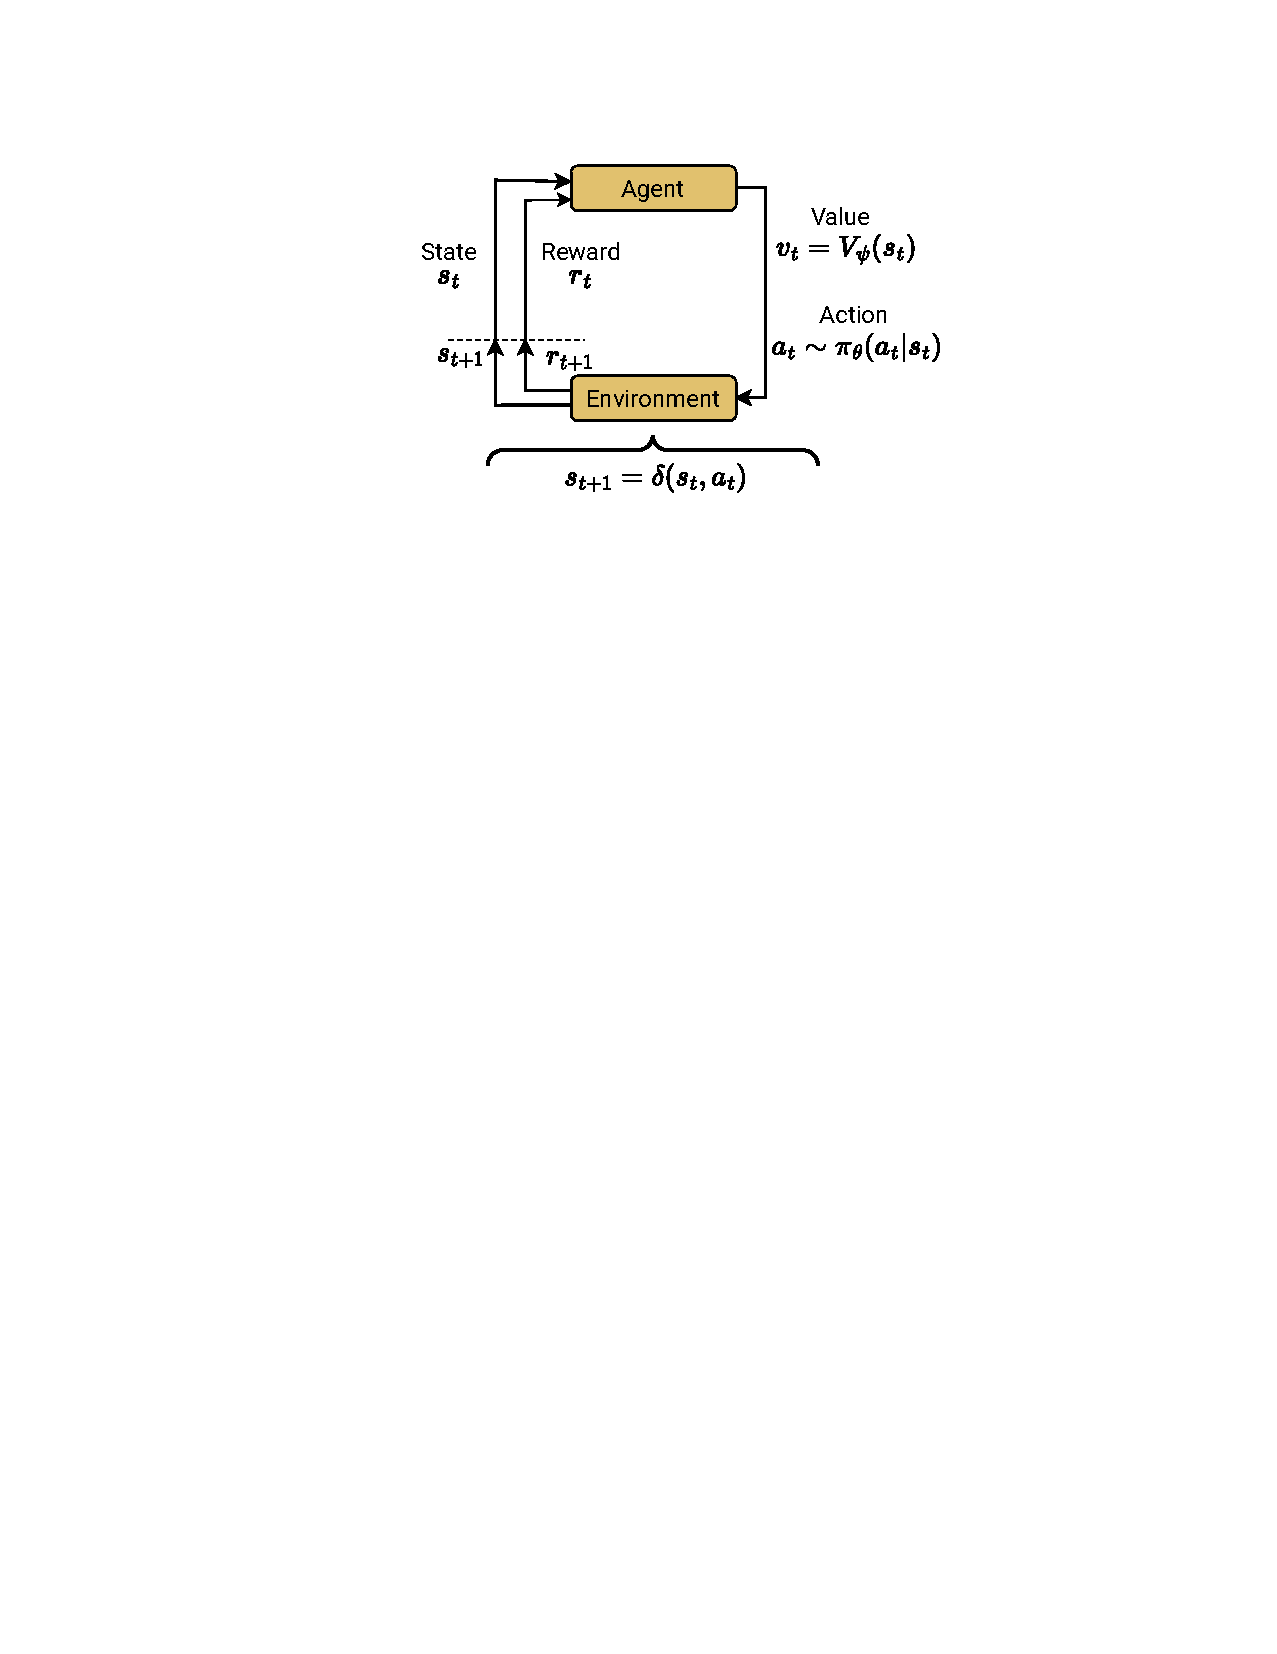
\includegraphics[clip, trim=7cm 19cm 5cm 2cm, width=1.3\textwidth]{rl.pdf}
  \end{figure}
   \tikzset{person/.style={draw,rectangle,fill=tab20darkgreen!60,rounded corners,inner sep=5pt} }
  \tikzset{object/.style={draw,rectangle,fill=tab20darkblue!60,rounded corners, inner sep=5pt, minimum height=0.7cm}}
  \tikzset{type/.style={draw,rectangle,fill=lightgray,inner sep=5pt}}
  \tikzset{>=triangle 45}
  \tikzset{every picture/.style=thick}
  \tikzstyle{every node}=[font=\small]
    \tikzstyle{arrow} = [->, thick,>=stealth']
  
  
  \vspace{-0.5cm}
    \resizebox{1.1\textwidth}{!}{%
  \hspace{0.0cm}
  \begin{tikzpicture}
    \node[object] (P1) {sepsis};
    \node[object, right= 0.5cm of P1, label={-90:$\mathbf{a_t = e_{t+1}}$}] (P2) {anemia};
    \node[object, right= 0.5cm of P2] (P3) {ards};
    \node[right= 0.1cm of P3] (P4) {\large $\biggl\} \, \, A(s_t)$};
    
    \node[person, above=of P2, label={90:$\mathbf{e_t}$}] (T1) {pneumonia};

    \draw[arrow, line width=1.2pt] (T1) -- (P1);
    \draw[arrow, line width=1.2pt] (T1) -- (P2);
    \draw[arrow, line width=1.2pt] (T1) -- (P3);

  \end{tikzpicture}}
  \end{columns}
\end{frame}

\begin{frame}{Agent}{Training}

\begin{itemize}
  \item Network Architecture
  \begin{itemize}
    \item LSTM to include the \emph{path history}
    \item Stack two feedforward networks on top\\$\Rightarrow$ For policy network and value network
  \end{itemize}

  \item<2-> Preprocessing of questions
  \begin{itemize}
    \item \emph{No negative information} in CauseNet\\$\Rightarrow$ Only use \emph{positive questions}
    \item Find $e_c$ and $e_e$ in graph via exact string matching
  \end{itemize}
  \item<3-> Sample rollouts
  \begin{itemize}
    \item Starting at $e_c$ sample \emph{rollouts of length $T$}
    \item If $e_e$ found, the agent should use the \textit{STAY} action
  \end{itemize}

  \begin{equation*}
    \uncover<3->{\text{rollout} = (} \uncover<4->{(s_0, a_0, r_0),} \uncover<5->{(s_1, a_1, r_1),} \uncover<6->{(s_2, a_2, r_2))}
  \end{equation*}
   \tikzset{person/.style={draw,rectangle,fill=tab20darkgreen!60,rounded corners,inner sep=5pt, minimum height=0.7cm} }
  \tikzset{object/.style={draw,rectangle,fill=tab20darkgreen!60,rounded corners, inner sep=5pt, minimum height=0.7cm}}
  \tikzset{type/.style={draw,rectangle,fill=lightgray,inner sep=5pt}}
  \tikzset{>=triangle 45}
  \tikzset{every picture/.style=thick}
  \tikzstyle{every node}=[font=\small]
    \tikzstyle{arrow} = [->, thick,>=stealth']

  \begin{textblock*}{5cm}(9.3cm,2.8cm) 
  \resizebox{0.65\textwidth}{!}{
  \begin{tikzpicture}[remember picture]
    %\node[object, xshift=2cm,yshift=2cm, anchor=north east] (P1) {organ failure};
    \uncover<5->{\node[object,xshift=2cm,yshift=2cm, anchor=north east, label={0:$\mathbf{s_2}, \mathbf{r_1 = 0}$}] (P2) {kidney failure};}
    %\node[object, right= 0.5cm of P2] (P3) {ards};
    
    \uncover<4->{\node[person, above=0.7cm of P2, label={0:$\mathbf{s_1}, \mathbf{r_0 = 0}$}] (T1) {sepsis};}
    \uncover<3->{\node[person, above=0.7cm of T1, label={0:$\mathbf{s_0}$}] (T2) {pneumonia};}
    %\node[person, below=0.7cm of P3] (T3) {death};
    \uncover<6->{\node[person, below=0.7cm of P2, label={0:$\mathbf{s_3}, \mathbf{r_2 = ?}$}] (T4) {anemia};}

    %\draw[->] (T1) -- (P1);
    \uncover<5->{\draw[arrow, line width=1.2pt] (T1) to node[right=0.04cm, pos=0.5]  {$\mathbf{a_1}$} (P2);}
    %\draw[->] (T1) -- (P3);
    \uncover<4->{\draw[arrow, line width=1.2pt] (T2) to node[right=0.04cm, pos=0.5]  {$\mathbf{a_0}$} (T1);}
    %\draw[->] (P3) -- (T3);
    \uncover<6->{\draw[arrow, line width=1.2pt] (P2) to node[right=0.04cm, pos=0.5]  {$\mathbf{a_2}$} (T4);}

  \end{tikzpicture}}
  \end{textblock*}
\end{itemize}


\end{frame}

\begin{frame}{Agent}{Update Rules}

\begin{itemize}
\item Using Synchronous Advantage Actor-Critic (A2C) with GAE
\item \emph{Actor:} policy network $\pi_{\theta}(a_t | s_t)$:
\begin{equation*}
  \nabla_{\theta} J(\theta) = - \frac{1}{B} \sum_{i}^{B} \sum_{t=0}^{T-2} \nabla_{\theta} \log(\pi_{\theta} (a_t | s_t)) \, \mathcal{A}_{t}^{\psi} + \beta H_{\pi_{\theta}}
\end{equation*}
  \begin{itemize}
  \item $B$: batch size, $T$: episode length, $\mathcal{A}_t^{\psi}$: GAE
  \item $H_{\pi_{\theta}}$: entropy regularization $\Rightarrow$ \emph{exploration vs. exploitation}
  \end{itemize}
\item<2-> \emph{Critic:} value network $V_{\psi}(s_t)$:
  \begin{equation*}
    \nabla_{\psi} J(\psi)= \frac{1}{B (T-1)} \sum_{i}^{B} \sum_{t=0}^{T-2} \nabla_{\psi} (R_t(\lambda) - V_{\psi}(s_t))^2
  \end{equation*}
  \begin{itemize}
  \item MSE between $\lambda$-return and value network predictions $V_{\psi}(s_t)$
  \end{itemize}
\end{itemize}
\end{frame}

\begin{frame}{Agent}{Inference}

\begin{block}{Inference Time}
  \begin{itemize}
  \item Receive positive and negative questions
  \item Answer ``yes'' if a path was found and ``no'' otherwise
  \end{itemize}
\end{block}

\vspace{-0.2cm}
\begin{itemize}
  \item<2-> Greedy decoding:
  \begin{itemize}
    \item Choose action: $arg\,max_{a_t \in \mathcal{A}(s_t)} \ \pi_{\theta}(a_t | s_t)$
    \item \emph{Myopic} behavior
  \end{itemize}
  \item<3-> Beam search:
  \begin{itemize}
    \item Always keep set of best partial solutions (paths)
    \item Paths \emph{ranked by their probability}
    \item Probability of path $p = (e_c,e_1, \dots, e_{T-1})$ with $e_t = a_{t-1}$:
    \begin{equation*}
  \mathbb{P}(p) = \prod_{t=0}^{T-2} \pi_{\theta}(a_t |s_t)
      \end{equation*}
  \end{itemize}
   \tikzset{person/.style={draw,rectangle,fill=tab20darkgreen!60,rounded corners,inner sep=5pt} }
  \tikzset{object/.style={draw,rectangle,fill=tab20darkblue!60,rounded corners, inner sep=5pt, minimum height=0.7cm}}
  \tikzset{type/.style={draw,rectangle,fill=lightgray,inner sep=5pt}}
  \tikzset{>=triangle 45}
  \tikzset{every picture/.style=thick}
  \tikzstyle{every node}=[font=\small]
    \tikzstyle{arrow} = [->, thick,>=stealth']
  
  
  \vspace{-0.5cm}
  \begin{textblock*}{5cm}(9cm,4.0cm) 
    \resizebox{0.65\textwidth}{!}{%
  \hspace{0.0cm}
  \begin{tikzpicture}
    \uncover<2->{\node[object, fill=white] (P1) {sepsis};}
    \uncover<2->{\node[object, right= 0.5cm of P1] (P2) {anemia};}
    \uncover<2->{\node[object, right= 0.5cm of P2, fill=white] (P3) {ards};}
    
    \uncover<2->{\node[person, above=of P2] (T1) {pneumonia};}

    \uncover<2->{\draw[arrow, line width=1.2pt] (T1) to node[left=0.04cm, pos=0.5]  {$0.2$} (P1);}
    \uncover<2->{\draw[arrow, line width=1.2pt] (T1) to node[right=0.00cm, pos=0.5]  {$\mathbf{0.6}$} (P2);}
    \uncover<2->{\draw[arrow, line width=1.2pt] (T1) to node[right=0.04cm, pos=0.5]  {$0.2$} (P3);}

  \end{tikzpicture}}
  \end{textblock*}
\end{itemize}

\end{frame}

\begin{frame}{Walkthrough}{Beam Width = 2}
\begin{figure}
    \centering
    \small
    \begin{tikzpicture}
        %\tikzstyle{vertex}=[draw, rectangle, rounded corners, minimum width=1.8cm, minimum height=1.4cm, line width=0.8pt]
        \tikzstyle{vertex}=[draw, rounded corners, line width=0.8pt, inner sep=4pt, minimum height = 0.7cm]
        \tikzstyle{box}=[minimum height=0.8cm, minimum width = 6cm, inner sep=4pt, rounded corners]
        \tikzstyle{arrow} = [->, thick,>=stealth']
        
        
        %\node[draw, line width=1pt] (Corner) {};
        \node[vertex] (N1) {bacteria};
        \node[vertex, left = 1.3cm of N1] (myocarditis) {myocarditis};
        \node[vertex, below = 1cm of myocarditis] (arrhythmia) {arrhythmia};
        \node[vertex, above left = 1.02cm and 1.32cm of N1] (pericarditis) {pericarditis};
        \node[vertex, above = 1cm of pericarditis] (pain) {pain};
        \node[vertex, right = 1cm of N1, fill=tab20darkgreen!60] (pneumonia) {pneumonia};
        \node[vertex, right = 1cm of pneumonia] (hospitalization) {hospitalization};
        \node[vertex, right = 0.8cm of hospitalization] (infections) {infections};
        \node[vertex, above = 1cm  of pneumonia, fill=tab20darkblue!60] (sepsis) {sepsis};
        \node[vertex, above = 1cm of sepsis] (hypoglycemia) {hypoglycemia};
        \node[vertex, left = 1.035cm of sepsis] (organ) {organ failure};
        \node[vertex, below = 1cm of pneumonia] (ards) {ards};
        \node[vertex, right = 1cm of ards] (death) {death};
        \node[vertex, right = 1cm of death] (grief) {grief};
        
        \node[vertex, right = 1cm  of sepsis, fill=tab20darkblue!60] (kidney) {kidney failure};
        \node[vertex, above = 1cm  of kidney] (bone) {bone pain};
        \node[vertex, right = 1cm  of kidney, fill=tab20darkblue!60] (anemia) {anemia};
        \node[vertex, above = 1cm  of anemia] (fatigue) {fatigue};
        
         \node[draw, rounded corners, line width=0.5pt, inner sep=4pt,below left = 0.8cm and -1.5cm of ards, fill=brass!60, minimum height=2cm, minimum width = 2.4cm, align=center] (LM) {Language \\ Model};
         
        \node[box, fill=brass!40, label=left:{}, above right = 4.1cm and -1.5cm of N1] (MCQ)  {\textbf{Question:} Can pneumonia cause anemia?};
         
         \node[left color=white, right color=brass!40, above left = -1.15cm and 0cm of LM, fill=brass!40, minimum height=1.1cm, minimum width = 4cm, align=center] (q1) {Can pneumonia cause ..};
         \node[left color=white, right color=brass!40, below = 0.1cm of q1, fill=brass!40, minimum height=0.73cm, minimum width = 4cm, align=center] (q2) {Colored Path};
         \node[left = 0.2cm of q1, fill=white, minimum height=1.1cm, minimum width = 1.5cm, align=center] (t1) {\textbf{Question:}};
         \node[left = 0.2cm of q2, fill=white, minimum height=1.1cm, minimum width = 1.5cm, align=center] (t2) {\textbf{Context:}};
         \node[right color=white, left color=brass!40, right = 0cm of LM, fill=brass!40, minimum height=1.4cm, minimum width = 4cm, align=center] (q3) {Yes, pneumonia can induce sepsis which ..};

        
        %\node[above left = 0.3cm and -0.4cm of pericarditis] (a) {\textbf{a)}};
        %\node[above left = 0.2cm and -0.5cm of MCQ] (b) {\textbf{b)}};
        %\node[below left = 0.35cm and 3.4cm of ards] (c) {\textbf{c)}};

        %\node[left = 0.1cm of sepsis] (ps) {\textbf{0.7}};
        %\node[above = 0.1cm of pneumonia] (pf) {\textbf{0.1}};
        %\node[left = 0.1cm of ards] (pa) {\textbf{0.2}};
        %\node[above = 0.1cm of death] (pa) {\textbf{1.0}};
        %\node[above = 0.1cm of kidney] (ph) {\textbf{1.0}};
        
        \draw[arrow, line width=1.2pt] (N1) -- (myocarditis);
        \draw[arrow, line width=1.2pt] (N1) -- (organ);
        \draw[arrow, line width=1.2pt] (pneumonia) to node[right=0.1cm, pos=0.5]  {$\mathbf{0.6}$} (sepsis);
        \draw[arrow, line width=1.2pt] (pneumonia)  to node[right=0.1cm, pos=0.5]  {$\mathbf{0.2}$}(ards);
        \draw[arrow, line width=1.2pt] (pneumonia) to node[above=0.1cm, pos=0.5]  {$\mathbf{0.15}$} (hospitalization);
        \draw[arrow, line width=1.2pt] (N1) to node[above=0.1cm, pos=0.5]  {$\mathbf{0.15}$} (pneumonia);
        \draw[arrow, line width=1.2pt] (kidney) to node[above=0.1cm, pos=0.5]  {$\mathbf{0.8}$} (anemia);
        \draw[arrow, line width=1.2pt] (kidney) to node[right=0.1cm, pos=0.5]  {$\mathbf{0.2}$} (bone);
        \draw[arrow, line width=1.2pt] (anemia) -- (fatigue);
        \draw[arrow, line width=1.2pt] (hospitalization) -- (infections);
        \draw[arrow, line width=1.2pt] (sepsis) to node[right=0.1cm, pos=0.5]  {$\mathbf{0.1}$} (hypoglycemia);
        \draw[arrow, line width=1.2pt] (sepsis) to node[above=0.1cm, pos=0.5]  {$\mathbf{0.2}$} (organ);
        \draw[arrow, line width=1.2pt] (myocarditis) -- (pericarditis);
        \draw[arrow, line width=1.2pt] (myocarditis) -- (arrhythmia);
        \draw[arrow, line width=1.2pt] (pericarditis) -- (pain);
        
        \draw[arrow, line width=1.2pt] (sepsis) to node[above=0.1cm, pos=0.5]  {$\mathbf{0.7}$} (kidney);
        \draw[arrow, line width=1.2pt] (ards) to  node[above=0.1cm, pos=0.5]  {$\mathbf{1.0}$} (death);
        \draw[arrow, line width=1.2pt] (death) to  node[above=0.1cm, pos=0.5]  {$\mathbf{1.0}$} (grief);

        \draw [draw, line width=1.2pt] (-5,5.5) -- (10,5.5);
        \draw [draw, line width=1.2pt] (-5,4.3) -- (10,4.3);
        \draw [draw, line width=1.2pt] (-5,-2.5) -- (10,-2.5);
        \draw [draw, line width=1.2pt] (-5,-5.25) -- (10,-5.25);
        %\draw[thick,rounded corners]     ($(inflammation.north west)+(-0.2,0.89)$) rectangle ($(death.south east)+(0.5,-0.3)$);
        
        %\draw[thick,rounded corners]     ($(ards.south west)+(-4,-0.3)$) rectangle ($(C.south east)+(0.5,-3)$);
    \end{tikzpicture}
    \caption{An excerpt from CauseNet~\cite{Heindorf2020Causenet} showing the entity \textit{pneumonia} together with its neighborhood containing causes and effects. 
            Each edge depicts a \textit{cause} relation. Given the question \textit{``Can pneumonia cause anemia?''}, the search
            starts at the entity \textit{pneumonia}. Following the path \textit{(pneumonia, sepsis, kidney failure, anemia)}, the question 
            can be answered with ``yes''. The numbers on the edges show the probability of taking this edge under the current 
            policy $\pi_{\theta}(a_t | s_t)$. For brevity, we only show the relevant probabilities for the given path. The lower part of the figure shows the possibility to combine our agent with a language model. In that setup, we provide the paths the agent learned for a question as additional context 
            to the language model. We briefly explore this setup in Section~\ref{sec:evaluation-approach}.
            }
    \label{fig:graph_example}
\end{figure}
\end{frame}

\begin{frame}{Bootstrapping with Supervised Learning}

\begin{itemize}
  \item Problem: large action space + sparse rewards
  \begin{itemize}
    \item \emph{Slow convergence}
    \item Guidance in the beginning
  \end{itemize}
  \item<2-> Generating expert demonstrations~{\scriptsize\cite{Xiong2017DeePpath}}:
  \begin{itemize}
    \item Paths from a \emph{breadth-first search (BFS)}
    \item Preprocessing step for each question $q$\\\textcolor{gray}{Find path between $e_c$ and $e_e$}
  \end{itemize}
  \item<3-> Supervised gradient update:
  \begin{itemize}
    \item \emph{$r_t = 1$ at each time step}
    \item Batch size $B$, episode length $T$
    \item Entropy regularization $H_{\pi_{\theta}}$
  \end{itemize}

    \begin{equation*}
      \nabla_{\theta} J(\theta) = - \frac{1}{B} \sum_{i}^{B} \sum_{t=0}^{T-2} \nabla_{\theta} \log(\pi_{\theta} (a_t | s_t)) \, r_t + \beta H_{\pi_\theta}
    \end{equation*}

   \tikzset{person/.style={draw,rectangle,fill=tab20darkgreen!60,rounded corners,inner sep=5pt, minimum height=0.7cm} }
  \tikzset{object/.style={draw,rectangle,fill=tab20darkgreen!60,rounded corners, inner sep=5pt, minimum height=0.7cm}}
  \tikzset{type/.style={draw,rectangle,fill=lightgray,inner sep=5pt}}
  \tikzset{>=triangle 45}
  \tikzset{every picture/.style=thick}
  \tikzstyle{every node}=[font=\small]
    \tikzstyle{arrow} = [->, thick,>=stealth']

  \begin{textblock*}{5cm}(9cm,1.8cm) 
  \resizebox{0.65\textwidth}{!}{
  \begin{tikzpicture}[remember picture]
    %\node[object, xshift=2cm,yshift=2cm, anchor=north east] (P1) {organ failure};
    \uncover<2->{\node[object,xshift=2cm,yshift=2cm, anchor=north east, label={0:$\mathbf{s_2}, \mathbf{r_1 = 1}$}] (P2) {kidney failure};}
    %\node[object, right= 0.5cm of P2] (P3) {ards};
    
    \uncover<2->{\node[person, above=0.7cm of P2, label={0:$\mathbf{s_1}, \mathbf{r_0 = 1}$}] (T1) {sepsis};}
    \uncover<2->{\node[person, above=0.7cm of T1, label={0:$\mathbf{s_0}$}] (T2) {pneumonia};}
    %\node[person, below=0.7cm of P3] (T3) {death};
    \uncover<2->{\node[person, below=0.7cm of P2, label={0:$\mathbf{s_3}, \mathbf{r_2 = 1}$}] (T4) {anemia};}

    %\draw[->] (T1) -- (P1);
    \uncover<2->{\draw[arrow, line width=1.2pt] (T1) to node[right=0.04cm, pos=0.5]  {$\mathbf{a_1}$} (P2);}
    %\draw[->] (T1) -- (P3);
    \uncover<2->{\draw[arrow, line width=1.2pt] (T2) to node[right=0.04cm, pos=0.5]  {$\mathbf{a_0}$} (T1);}
    %\draw[->] (P3) -- (T3);
    \uncover<2->{\draw[arrow, line width=1.2pt] (P2) to node[right=0.04cm, pos=0.5]  {$\mathbf{a_2}$} (T4);}

  \end{tikzpicture}}
  \end{textblock*}
\end{itemize}

\end{frame}


\begin{frame}{Reward Shaping}

\begin{itemize}
    \item Problem: sparse rewards
    \begin{itemize}
      \item Agent only receives a reward if $e_{T-1} = e_e$
      \item Rarely finds correct paths at the start
    \end{itemize}
    \item<2-> Introduce \emph{auxiliary reward}:
    \begin{itemize}
      \item Score \emph{last node} according to its \emph{relevance}\\to the question~{\scriptsize\cite{Yasunaga2021QAGNN}}
    \end{itemize}
    \item<3-> Updated reward:
    \begin{equation*}
      \mathcal{R}'(s_{T-1}) =
        \begin{cases}
          \mathcal{R}(s_{T-1}), & \mathcal{R}(s_{T-1}) = 1 \\
          Score(q, e_{T-1}) \cdot \omega, & \text{otherwise}
        \end{cases}
    \end{equation*}
    \item<3-> Where $Score$ is defined as:
    \begin{equation*}
      Score(q, e_{T-1}) = LM_{head}(LM_{enc}([q;e_{T-1}]))
    \end{equation*}
    \vspace{-0.5cm}
    \begin{itemize}
    \item $LM_{head}$: feedforward network, $LM_{enc}$: language model encoder
    \end{itemize}
\end{itemize}

   \tikzset{person/.style={draw,rectangle,fill=tab20darkgreen!60,rounded corners,inner sep=5pt, minimum height=0.7cm} }
  \tikzset{object/.style={draw,rectangle,fill=tab20darkgreen!60,rounded corners, inner sep=5pt, minimum height=0.7cm}}
  \tikzset{type/.style={draw,rectangle,fill=lightgray,inner sep=5pt}}
  \tikzset{>=triangle 45}
  \tikzset{every picture/.style=thick}
  \tikzstyle{every node}=[font=\small]
  \tikzstyle{arrow} = [->, thick,>=stealth']
  \tikzstyle{box}=[minimum height=0.8cm, minimum width = 6cm, inner sep=4pt, rounded corners]

  \begin{textblock*}{5cm}(9cm,1.8cm) 
  \resizebox{0.7\textwidth}{!}{
  \begin{tikzpicture}[remember picture]
    %\node[object, xshift=2cm,yshift=2cm, anchor=north east] (P1) {organ failure};
    \uncover<2->{\node[object,xshift=2cm,yshift=2cm, anchor=north east, fill=tab20darkred!60,label={0: \huge $\mathbf{\downarrow}$}] (P2) {climate change};}
    %\node[object, right= 0.5cm of P2] (P3) {ards};
    
    \uncover<2->{\node[person, above=0.7cm of P2, label={0: \huge $\mathbf{\uparrow}$}] (T1) {sepsis};}
    \uncover<2->{\node[above=0.7cm of T1] (T2) {\textbf{Does pneumonia cause anemia?}};}

  \end{tikzpicture}}
  \end{textblock*}
\end{frame}

\begin{frame}{Evaluation}



\begin{center}
\footnotesize
  \renewcommand{\arraystretch}{0.95}
  \renewcommand{\tabcolsep}{6.4pt}
  \begin{tabular}{lccccr} 
    \toprule
    \multicolumn{6}{c}{\textbf{MS MARCO}}\\
    \midrule
    & \textbf{Accuracy} & \textbf{$\mathbf{F_1}$} & \textbf{Recall} & \textbf{Precision} & \textbf{|Nodes|}\\
    \midrule
    %Agent 1-Hop & 0.36 & & \\
    Agent 2-Hop & 0.460 & 0.562 & 0.408 & \textbf{0.901} & \textbf{26}\\
    Agent 3-Hop & 0.529 & 0.648 & 0.511 & 0.884 & 27 \\
    \midrule
    %BFS 1-Hop & 0.259 & 0.241 & 0.139 & \textbf{0.912} & 57 \\ 
    BFS 2-Hop & 0.494 & 0.612 & 0.471 & 0.875 & 1,727 \\ 
    BFS 3-Hop & 0.589 & 0.714 & 0.605 & 0.871 & 3,339\\ 
    \midrule
    UnifiedQA-v2 & \textbf{0.722} & \textbf{0.828} & \textbf{0.789} & 0.871 & -- \\
    %UnifiedQA-v2 | CauseNet 3-Hop & 0.787 & 0.877 & 0.897 & 0.858 & --  \\
    %UnifiedQA-v2 | Agent 3-Hop & 0.779 & 0.872 & 0.883 & 0.860 & -- \\
    %UnifiedQA-v2 --- Context & 0.661 & 0.789 & 0.740 & 0.842 & --\\
    %\midrule
    %Majority Baseline (True) & 0.848  & 0.9177 & 1.000 & 0.848 & --\\
    \bottomrule
\end{tabular}
%\end{table}
%\begin{table}[t]
\centering
\renewcommand{\tabcolsep}{6.47pt}
\hspace{-0.20cm}
%\caption{Evaluation SemEval.}
\begin{tabular}{lccccr} 
    \toprule
    \multicolumn{6}{c}{\textbf{SemEval}}\\
    \midrule
    & \textbf{Accuracy} & \textbf{$\mathbf{F_1}$} & \textbf{Recall} & \textbf{Precision} & \textbf{|Nodes|}\\
    \midrule
    %Agent 1-Hop & 0.36 & & \\
    Agent 2-Hop &  0.769 & 0.714 & 0.575 & \textbf{0.943} & \textbf{27}\\
    Agent 3-Hop & 0.775 & 0.727 & 0.598 & 0.929 & 29\\
    \midrule
    %BFS 1-Hop & 0.665 & 0.508 & 0.345 & \textbf{0.968} & 35 \\ 
    BFS 2-Hop & \textbf{0.815} & \textbf{0.787} & 0.678 & 0.937 & 1,565 \\ 
    BFS 3-Hop & 0.751 & 0.754 & 0.759 & 0.750 & 3,687\\ 
    \midrule
    UnifiedQA-v2 & 0.497 & 0.653 & \textbf{0.943} & 0.500 & --\\
    %UnifiedQA-v2 | CauseNet 3-Hop & 0.520 & 0.677 & 1.000 & 0.512 & -- \\
    %UnifiedQA-v2 | Agent 3-Hop & 0.520 & 0.675 & 0.989 & 0.512 & -- \\
    %UnifiedQA-v2 --- Context & 0.566 & 0.651 & 0.805 & 0.547 & -- \\
    %\midrule
    %Majority Baseline (True) & 0.503 & 0.669 & 1.000 & 0.503 & -- \\
    \bottomrule
\end{tabular}
\end{center}



\end{frame}


\begin{frame}{Ablation Study}

\begin{center}
  \setlength{\tabcolsep}{2pt}
  \renewcommand{\arraystretch}{1.08}
  \footnotesize
  \begin{tabular}{lcccccccc} 
		\toprule
		& \multicolumn{4}{c}{\textbf{MS MARCO}} & \multicolumn{4}{c}{\textbf{SemEval}}  \\
		\cmidrule(lr{.6em}){2-5} \cmidrule(l{0.3em}){6-9}
		&\textbf{A} & \textbf{$\mathbf{F_1}$} & \textbf{R} & \textbf{P} & \textbf{A} & \textbf{$\mathbf{F_1}$} & \textbf{R} & \textbf{P}\\
		\midrule
		Agent 2-Hop & \textbf{0.460} & \textbf{0.562} & \textbf{0.408} & 0.901 & \textbf{0.769} & \textbf{0.714} & \textbf{0.575} & 0.943 \\ 
		\midrule
		$\mathbf{-}$ Beam Search & 0.293 & 0.306 &0.184 & \textbf{0.911} & 0.613 & 0.374 &0.230& \textbf{1.000} \\
		$\mathbf{-}$ Supervised Learning & 0.342 & 0.397 & 0.257 & 0.891 & 0.682 & 0.538 & 0.369 & \textbf{1.000} \\
		$\mathbf{-}$ Actor-Critic & 0.441 & 0.539 & 0.386 & 0.896 & 0.740 & 0.657 &0.494& 0.977 \\
		$\mathbf{-}$ Inverse Edges & 0.422 & 0.513 &0.359& 0.899 & 0.740 & 0.651 & 0.483 & \textbf{1.000} \\
		$\mathbf{+}$ Reward Shaping (0.1) & 0.449 & 0.548 & 0.395 & 0.898 & 0.757 & 0.691 & 0.540 & 0.959 \\
		$\mathbf{+}$ Reward Shaping (1.0) & 0.403 &0.489 & 0.336 & 0.893 & \textbf{0.769} & 0.706 & 0.552 & 0.980 \\
		\bottomrule
	\end{tabular}
\end{center}

%\begin{itemize}
  %\item Beam search most important
  %\item Beam search most important
%\end{itemize}

\end{frame}

\begin{frame}{Effects of Supervised Learning}{Accuracy}
\begin{figure}
	\centering

    \resizebox{0.9\textwidth}{!}{%
	\begin{tikzpicture}
		\begin{axis}
			[	%legend pos=outer north east,
				legend cell align={left},
				legend style={legend pos=south east},
				xlabel=steps,
				ylabel=accuracy,
				grid=major,
				xtick={0, 20, 40, 60, 80, 100, 120, 140, 160, 180, 200},
				xticklabels={0, 200 , 400, 600, 800, 1000, 1200, 1400, 1800, 1900, 2000},
				ytick={0.66, 0.68, 0.70, 0.72, 0.74, 0.76, 0.78, 0.80},
				yticklabels={0.66, 0.68, 0.70, 0.72, 0.74, 0.76, 0.78, 0.80},
				xmin=0,
				xmax=200,
				ymin=0.66,
				ymax=0.80,
				width=14cm,
				height=9cm]
			%\addplot[mark=none, tab20darkgreen, very thick] table [x=Step, y=r_semeval_400_1.0_32_5000_ff - accuracy, col sep=comma] {data/supervised_accuracy.csv};
			%\addlegendentry{400 Steps}
			\addplot[mark=none, tab20darkred, very thick] table [x=Step, y=r_semeval_300_1.0_32_5000_ff - accuracy, col sep=comma] {data/supervised_accuracy.csv};
			\addlegendentry{300 Steps}
			\addplot[mark=none, tab20darkblue, very thick] table [x=Step, y=r_semeval_200_1.0_32_5000_ff - accuracy, col sep=comma] {data/supervised_accuracy.csv};
			\addlegendentry{200 Steps}
			\addplot[mark=none, tab20darkorange, very thick] table [x=Step, y=r_semeval_100_1.0_32_5000_ff - accuracy, col sep=comma] {data/supervised_accuracy.csv};
			\addlegendentry{100 Steps}
		\end{axis}
	\end{tikzpicture}}
\end{figure}
\end{frame}

\begin{frame}{Effects of Supervised Learning}{Number of Explored Paths + Entropy of Policy Network}
\begin{figure}[ht]
	\begin{minipage}{.45\linewidth}
	  \centering
	\resizebox{1.26\textwidth}{!}{%
\begin{tikzpicture}
	\hspace{-1.5cm}
	\begin{axis}
		[	%legend pos=outer north east,
			legend cell align={left},
			legend style={legend pos=north west},
			xlabel=steps,
			ylabel=|paths|,
			%ylabel shift = 0.1 pt,
			scaled y ticks = false,
			grid=major,
			xtick={0, 50, 100, 150, 200},
			xticklabels={0, 500, 1000, 1500, 2000},
			ytick={0, 20000, 40000, 60000, 80000},
			yticklabels={0, 20000, 40000, 60000, 80000},
			xmin=0,
			xmax=200,
			ymin=0,
			ymax=80000,
			width=8cm,
			height=8cm]
		%\addplot[mark=none, tab20darkgreen, very thick] table [x=Step, y=r_semeval_400_1.0_32_5000_ff - unique_paths, col sep=comma] {data/supervised_paths.csv};
		%\addlegendentry{400 Steps}
		\addplot[mark=none, tab20darkred, very thick] table [x=Step, y=r_semeval_300_1.0_32_5000_ff - unique_paths, col sep=comma] {data/supervised_paths.csv};
		\addlegendentry{300 Steps}
		\addplot [mark=none, tab20darkblue, very thick]table [x=Step, y=r_semeval_200_1.0_32_5000_ff - unique_paths, col sep=comma] {data/supervised_paths.csv};
		\addlegendentry{200 Steps}
		\addplot [mark=none, tab20darkorange, very thick]table [x=Step, y=r_semeval_100_1.0_32_5000_ff - unique_paths, col sep=comma] {data/supervised_paths.csv};
		\addlegendentry{100 Steps}
		\addplot [mark=none, tab20darkgreen, very thick]table [x=Step, y=r_semeval_no_super_5000_ff - unique_paths, col sep=comma] {data/supervised_paths.csv};
		\addlegendentry{0 Steps}
	\end{axis}
\end{tikzpicture}}
	\end{minipage}
	%\hspace*{0.7cm}
	\begin{minipage}{.45\linewidth}
	  \centering
	\resizebox{1.2\textwidth}{!}{%
\begin{tikzpicture}
	\begin{axis}
		[	%legend pos=outer north east,
			legend cell align={left},
			legend style={legend pos=north east},
			xlabel=steps,
			ylabel=entropy,
			grid=major,
			xtick={0, 50, 100, 150, 200},
			xticklabels={0, 500, 1000, 1500, 2000},
			ytick={0.0, 0.5, 1.0, 1.5, 2.0, 2.5, 3.0, 3.5},
			yticklabels={0.0, 0.5, 1.0, 1.5, 2.0, 2.5, 3.0, 3.5},
			xmin=0,
			xmax=200,
			ymin=0.0,
			ymax=3.5,
			width=8cm,
			height=8cm]
		%\addplot[mark=none, tab20darkgreen, very thick] table [x=Step, y=r_semeval_400_1.0_32_5000_ff - entropy, col sep=comma] {data/supervised_entropy.csv};
		%\addlegendentry{400 Steps}
		\addplot[mark=none, tab20darkred, very thick] table [x=Step, y=r_semeval_300_1.0_32_5000_ff - entropy, col sep=comma] {data/supervised_entropy.csv};
		\addlegendentry{300 Steps}
		\addplot [mark=none, tab20darkblue, very thick]table [x=Step, y=r_semeval_200_1.0_32_5000_ff - entropy, col sep=comma] {data/supervised_entropy.csv};
		\addlegendentry{200 Steps}
		\addplot [mark=none, tab20darkorange, very thick]table [x=Step, y=r_semeval_100_1.0_32_5000_ff - entropy, col sep=comma] {data/supervised_entropy.csv};
		\addlegendentry{100 Steps}
		\addplot[mark=none, tab20darkgreen, very thick] table [x=Step, y=r_semeval_no_super_5000_ff - entropy, col sep=comma] {data/supervised_entropy.csv};
		\addlegendentry{0 Steps}
	\end{axis}
\end{tikzpicture}}
	\end{minipage}
  \end{figure}
\end{frame}

\begin{frame}{Conclusion}
\begin{itemize}
    \item Summary
    \begin{itemize}
        \item Introduced an Actor-Critic (A2C) based agent\\to answer causal questions
        \item Extended with supervised learning and reward shaping
    \end{itemize}
    \item<2-> Conclusion
    \begin{itemize}
        \item Supervised learning provides an effective foundation
        \item Effectively \emph{prunes the search space by around 99\%}
        \item Paths can be used as \emph{explanations}\\$\Rightarrow$ Use meta-information to \emph{verify the claims}
    \end{itemize}
    \item<3-> Future Work
    \begin{itemize}
        \item Extend to \emph{open-ended questions}\\$\Rightarrow$Straightforward extension via majority voting
        \item Add different causal knowledge graphs
        \item Explore ways to consider negative\\causal questions during training
    \end{itemize}

   \tikzset{person/.style={draw,rectangle,fill=tab20darkgreen!60,rounded corners,inner sep=5pt, minimum height=0.7cm} }
  \tikzset{object/.style={draw,rectangle,fill=tab20darkgreen!60,rounded corners, inner sep=5pt, minimum height=0.7cm}}
  \tikzset{type/.style={draw,rectangle,fill=lightgray,inner sep=5pt}}
  \tikzset{>=triangle 45}
  \tikzset{every picture/.style=thick}
  \tikzstyle{every node}=[font=\small]
    \tikzstyle{arrow} = [->, thick,>=stealth']

  \begin{textblock*}{5cm}(9cm,3.8cm) 
  \resizebox{0.7\textwidth}{!}{
  \begin{tikzpicture}[remember picture]
    
    \node[object, xshift=2cm,yshift=2.2cm, anchor=north east] (P1) {fatigue};
    \node[object, right= 0.7cm of P1] (P2) {sepsis};
    \node[object, right= 0.7cm of P2] (P3) {ards};
    
    \node[person, above=0.7cm of P2] (T1) {pneumonia};
    \node[person, above=0.7cm of T1] (T2) {bacteria};
    \node[person, below=0.7cm of P3] (T3) {death};
    \node[person, below=0.7cm of T3] (P8) {grief};
    \node[person, below=0.7cm of P2] (T4) {kidney failure};
    \node[person, below=0.7cm of T4] (P7) {anemia};

    %\node[above=0.7cm of T2] (T5) {\textbf{Does pneumonia cause anemia?}};

    \draw[arrow, line width=1.2pt] (T1) -- (P1);
    \draw[arrow, line width=1.2pt] (T1) -- (P2);
    \draw[arrow, line width=1.2pt] (T1) -- (P3);
    \draw[arrow, line width=1.2pt] (T2) -- (T1);
    \draw[arrow, line width=1.2pt] (P3) -- (T3);
    \draw[arrow, line width=1.2pt] (P2) -- (T4);
    \draw[arrow, line width=1.2pt] (T4) -- (P7);
    \draw[arrow, line width=1.2pt] (T3) -- (P8);

  \end{tikzpicture}}
  \end{textblock*}
\end{itemize}
\end{frame}

\begin{frame}[allowframebreaks]{References}{~}
  \scriptsize
  \bibliographystyle{apalike}
  %\renewcommand{\bibfont}{\fontsize{8pt}{9pt}\selectfont}
  \bibliography{ref}
  
  \end{frame}

%\begin{frame}{Thank you!}
%\centering
%	\vspace{2.5cm}
%	{\huge\textbf{Questions?}}
%	\\\vspace{2.5cm}
%	{\large Data Science Group at Paderborn University}
%	\\\vspace{.1cm}
%	\centering
%	\begin{tabular}{rl}
%	Web: & \href{https://dice-research.org/}{dice-research.org} \\
%	Code: & \href{https://github.com/dice-group}{github.com/dice-group} \\
%	Twitter: & \href{https://twitter.com/DiceResearch}{@DiceResearch}
%	\end{tabular}
%\end{frame}

\begin{frame}{$\mathbf{\lambda}$-return \& GAE}
  \begin{itemize}
    \item N-step returns:
    \begin{equation*}
      R_t^{(n)} = \sum_{i=0}^{n-1} \gamma^i \, r_{t+i} + \gamma^n V_{\psi} (s_{t+n}) 
    \end{equation*}
    \item Which $n$ is best?
    \item $\lambda$-return exponentially-weighted average of $n$-step returns:
    \begin{equation*}
      %\vspace{-1cm}
      R_t(\lambda) = (1- \lambda) \sum_{n=1}^{\infty} \lambda^{n-1} R_t^{(n)} = (1-\lambda) \sum_{n=1}^{T-t-1} \lambda^{n-1} \, R_t^{(n)} + \lambda^{T-t-1} R_t^{(T-t)} 
    \end{equation*}
  \end{itemize}
\end{frame}

\begin{frame}{Network Architecture}
\begin{itemize}
    \item LSTM:
    \begin{equation*}
      \mathbf{h_t}=
        \begin{cases}
          LSTM(\mathbf{0}; [\mathbf{q}, \mathbf{e_c}]), & \text{if}\ t=0 \\
          LSTM(\mathbf{h_{t-1}}, [\mathbf{q}; \mathbf{e_t}]), & \text{otherwise}
        \end{cases}
    \end{equation*}
    \item Policy network $\pi_{\theta}(a_t | s_t)$:
    \begin{equation*}
      \begin{split}
      \pi_\theta(a_t | s_t) = \sigma(\mathbf{A_t} \times W_2 \times ReLU(W_1 \times \mathbf{h_t})) \\
      a_t \sim Categorical(\pi_\theta(a_t | s_t))
      \end{split}
    \end{equation*}
    \begin{itemize}
      \item $\mathbf{A_t} \in \mathcal{R}^{|A(s_t)| \times 2d}$ embeddings of actions $a_t \in \mathcal{A}(s_t)$
      \item $\sigma$: softmax operator
    \end{itemize}
    \item Value network $V_{\psi}(s_t)$:
    \begin{equation*}
      V_{\psi}(s_t) = W_4 \times ReLU(W_3 \times \mathbf{h_t})
    \end{equation*}

\end{itemize}
\end{frame}

\begin{frame}{Entropy}
  \begin{equation*}
    H_{\pi_\theta} = \frac{1}{B(T-1)} \sum_{i}^{B} \sum_{t=0}^{T-2} (- \hspace{-0.3cm}\sum_{a_t \in \mathcal{A}(s_t)} \pi_\theta(a_t | s_t)  \log \pi_\theta(a_t | s_t))
  \end{equation*}
\end{frame}

\begin{frame}{Beam Search Evaluation}
  \begin{figure}
    \centering
	\resizebox{1.0\textwidth}{!}{%
    \begin{tikzpicture}
      \begin{axis}
        [	%legend pos=outer north east,
          legend cell align={left},
          legend style={legend pos=south east},
          xlabel=steps,
          ylabel=accuracy,
          grid=major,
          xtick={0, 40, 80, 120, 160, 200, 240, 280, 320, 360, 400},
          xticklabels={0, 400, 800, 1200, 1600, 2000, 2400, 2800, 3200, 3600, 4000},
          ytick={0.1, 0.15, 0.2, 0.25, 0.3, 0.35, 0.4},
          yticklabels={0.1, 0.15, 0.2, 0.25, 0.3, 0.35, 0.4},
          xmin=0,
          xmax=400,
          ymin=0.1,
          ymax=0.4,
          width=14cm,
          height=8cm]
        \addplot [mark=none, tab20darkgreen, very thick]table [x=Step, y=r_msmarco_bm_50_5000_ff - accuracy, col sep=comma] {data/beam_path_inverse.csv};
        \addlegendentry{Width: 50}
        \addplot [mark=none, tab20darkorange, very thick]table [x=Step, y=r_msmarco_bm_10_5000_ff - accuracy, col sep=comma] {data/beam_path_inverse.csv};
        \addlegendentry{Width: 10}
        \addplot [mark=none, tab20darkblue, very thick]table [x=Step, y=r_msmarco_bm_5_5000_ff - accuracy, col sep=comma] {data/beam_path_inverse.csv};
        \addlegendentry{Width: 5}
        \addplot[mark=none, tab20darkred, very thick] table [x=Step, y=r_msmarco_bm_1_5000_ff - accuracy, col sep=comma] {data/beam_path_inverse.csv};
        \addlegendentry{Width: 1}
      \end{axis}
    \end{tikzpicture}}
    \end{figure}
\end{frame}

\begin{frame}{Inference Time}
  \begin{figure}[ht]
    \begin{minipage}{.45\linewidth}
      \centering
	\resizebox{1.16\textwidth}{!}{%
  \begin{tikzpicture}
    \hspace{-1.0cm}
    \begin{axis}
      [	%legend pos=outer north east,
        legend cell align={left},
        legend style={legend pos=north west},
        xlabel=beam width,
        ylabel=seconds,
        %ylabel shift = 0.1 pt,
        scaled y ticks = false,
        grid=major,
        xtick={1, 10, 20, 30, 40, 50},
        xticklabels={1, 10, 20, 30, 40, 50},
        ytick={0, 30, 60, 90, 120, 150, 180},
        ytick={0, 30, 60, 90, 120, 150, 180},
        extra x ticks={25},
        extra x tick labels={\textbf{MS MARCO}},
        extra x tick style={grid=none,ticks=major,ticklabel pos=right},
        xmin=1,
        xmax=50,
        ymin=0,
        ymax=180,
        width=8cm,
        height=8cm]
      \addplot[mark=none, tab20darkred, very thick] table [x=width, y=numbers, col sep=comma] {data/length2_msmarco.csv};
      \addlegendentry{Length: 2}
      \addplot [mark=none, tab20darkblue, very thick]table [x=width, y=numbers, col sep=comma] {data/length3_msmarco.csv};
      \addlegendentry{Length: 3}
    \end{axis}
  \end{tikzpicture}}
    \end{minipage}
    \hspace*{0.5cm}
    \begin{minipage}{.45\linewidth}
      \centering
	\resizebox{1.16\textwidth}{!}{%
  \begin{tikzpicture}
    \begin{axis}
      [	%legend pos=outer north east,
        legend cell align={left},
        legend style={legend pos=north west},
        xlabel=beam width,
        ylabel=seconds,
        grid=major,
        xtick={1, 10, 20, 30, 40, 50},
        xticklabels={1, 10, 20, 30, 40, 50},
        ytick={0, 30, 60, 90, 120, 150, 180},
        ytick={0, 30, 60, 90, 120, 150, 180},
        extra x ticks={25},
        extra x tick labels={\textbf{SemEval}},
        extra x tick style={grid=none,ticks=major,ticklabel pos=right},
        xmin=1,
        xmax=50,
        ymin=0,
        ymax=180,
        width=8cm,
        height=8cm]
      \addplot[mark=none, tab20darkred, very thick] table [x=width, y=numbers, col sep=comma] {data/length2_semeval.csv};
      \addlegendentry{Length: 2}
      \addplot [mark=none, tab20darkblue, very thick]table [x=width, y=numbers, col sep=comma] {data/length3_semeval.csv};
      \addlegendentry{Length: 3}
    \end{axis}
  \end{tikzpicture}}
    \end{minipage}
  \end{figure}
\end{frame}

\begin{frame}{Inverse Edges}
  \begin{itemize}
    \item Pro:
    \begin{itemize}
      \item Undo wrong actions
      \item Reach nodes that could otherwise not be reached in $T$ steps
    \end{itemize}
    \item Con:
    \begin{itemize}
      \item Introduction of false positives
      \item Atleast in theory it might not make sense to take an inverse edge
    \end{itemize}
    \item Does $e_1$ cause $e_4$? and $T = 2$:
  \end{itemize}
   \tikzset{person/.style={draw,rectangle,fill=tab20darkgreen!60,rounded corners,inner sep=5pt, minimum height=0.7cm} }
  \tikzset{object/.style={draw,rectangle,fill=tab20darkgreen!60,rounded corners, inner sep=5pt, minimum height=0.7cm}}
  \tikzset{type/.style={draw,rectangle,fill=lightgray,inner sep=5pt}}
  \tikzset{>=triangle 45}
  \tikzset{every picture/.style=thick}
  \tikzstyle{every node}=[font=\small]
    \tikzstyle{arrow} = [->, thick,>=stealth']

  %\begin{textblock*}{5cm}(9cm,1.8cm) 
  \begin{figure}
    \centering
  \resizebox{0.4\textwidth}{!}{
  \begin{tikzpicture}[remember picture]
    
    %\node[object, xshift=2cm,yshift=2.2cm, anchor=north east] (P1) {fatigue};
    \node[object, fill=tab20darkblue!60] (P1) {$e_1$};
    \node[object, right= 0.7cm of P1] (P2) {$e_2$};
    \node[object, right= 0.7cm of P2] (P3) {$e_3$};
    \node[object, right= 0.7cm of P3, fill=tab20darkblue!60] (P4) {$e_4$};
    \node[object, below= 0.7cm of P2, fill=tab20darkblue!60] (P5) {$e_5$};

    \draw[arrow, line width=1.2pt] (P1) -- (P2);
    \draw[arrow, line width=1.2pt] (P2) -- (P3);
    \draw[arrow, line width=1.2pt] (P3) -- (P4);
    \draw[arrow, line width=1.2pt] (P1) -- (P5);
    \draw[arrow, line width=1.2pt] (P4) -- (P5);

  \end{tikzpicture}}
\end{figure}
  %\end{textblock*}
\end{frame}

\begin{frame}{Examples}
  \begin{table}
    \centering
    \scriptsize
    \begin{tabular}{m{10cm} m{0.2cm}}
      \toprule
      \multicolumn{2}{c}{\textbf{Agent 3-Hop}} \\
      \midrule
       \vspace{0.2cm}
      \textbf{Cause:} h.\ pylori \hspace{0.54cm} \textbf{Effect:} vomiting &\\ 
       \vspace{0.2cm}
      \textbf{Path:} h.\ pylori $\xRightarrow{\text{cause}}$ peptic ulcer disease $\xRightarrow{\text{cause}}$ vomiting $\xRightarrow{\text{\textit{STAY}}}$ vomiting \vspace{0.2cm}\\
      \midrule
       \vspace{0.2cm}
      \textbf{Cause:} Xanax \hspace{0.92cm} \textbf{Effect:} hiccups &\\ 
       \vspace{0.2cm}
      \textbf{Path:} xanax $\xRightarrow{\text{cause}}$ anxiety $\xRightarrow{\text{cause}}$ stress $\xRightarrow{\text{cause}}$ hiccups \vspace{0.2cm}\\
      \midrule
       \vspace{0.2cm}
      \textbf{Cause:} chocolate \hspace{0.39cm} \textbf{Effect:} constipation &\\ 
       \vspace{0.2cm}
      \textbf{Path:} chocolate $\xRightarrow{\text{cause}}$ constipation $\xRightarrow{\text{cause}}$ depression $\xRightarrow{\text{cause}^{-1}}$ constipation \vspace{0.2cm}\\
      \midrule
       \vspace{0.2cm}
      \textbf{Cause:} rainfall \hspace{0.80cm} \textbf{Effect:} flooding &\\ 
       \vspace{0.2cm}
      \textbf{Path:} rainfall $\xRightarrow{\text{cause}}$ flooding $\xRightarrow{\text{cause}}$ landslides $\xRightarrow{\text{\textit{STAY}}}$ landslides \vspace{0.2cm}\\
      \bottomrule
    \end{tabular}
    \end{table}
\end{frame}

\end{document}